\section{Spark::Sp\-Matrix2$<$ Real $>$ Class Template Reference}
\label{classSpark_1_1SpMatrix2}\index{Spark::SpMatrix2@{Spark::SpMatrix2}}
{\tt \#include $<$Sp\-Matrix.h$>$}

Inheritance diagram for Spark::Sp\-Matrix2$<$ Real $>$:\begin{figure}[H]
\begin{center}
\leavevmode
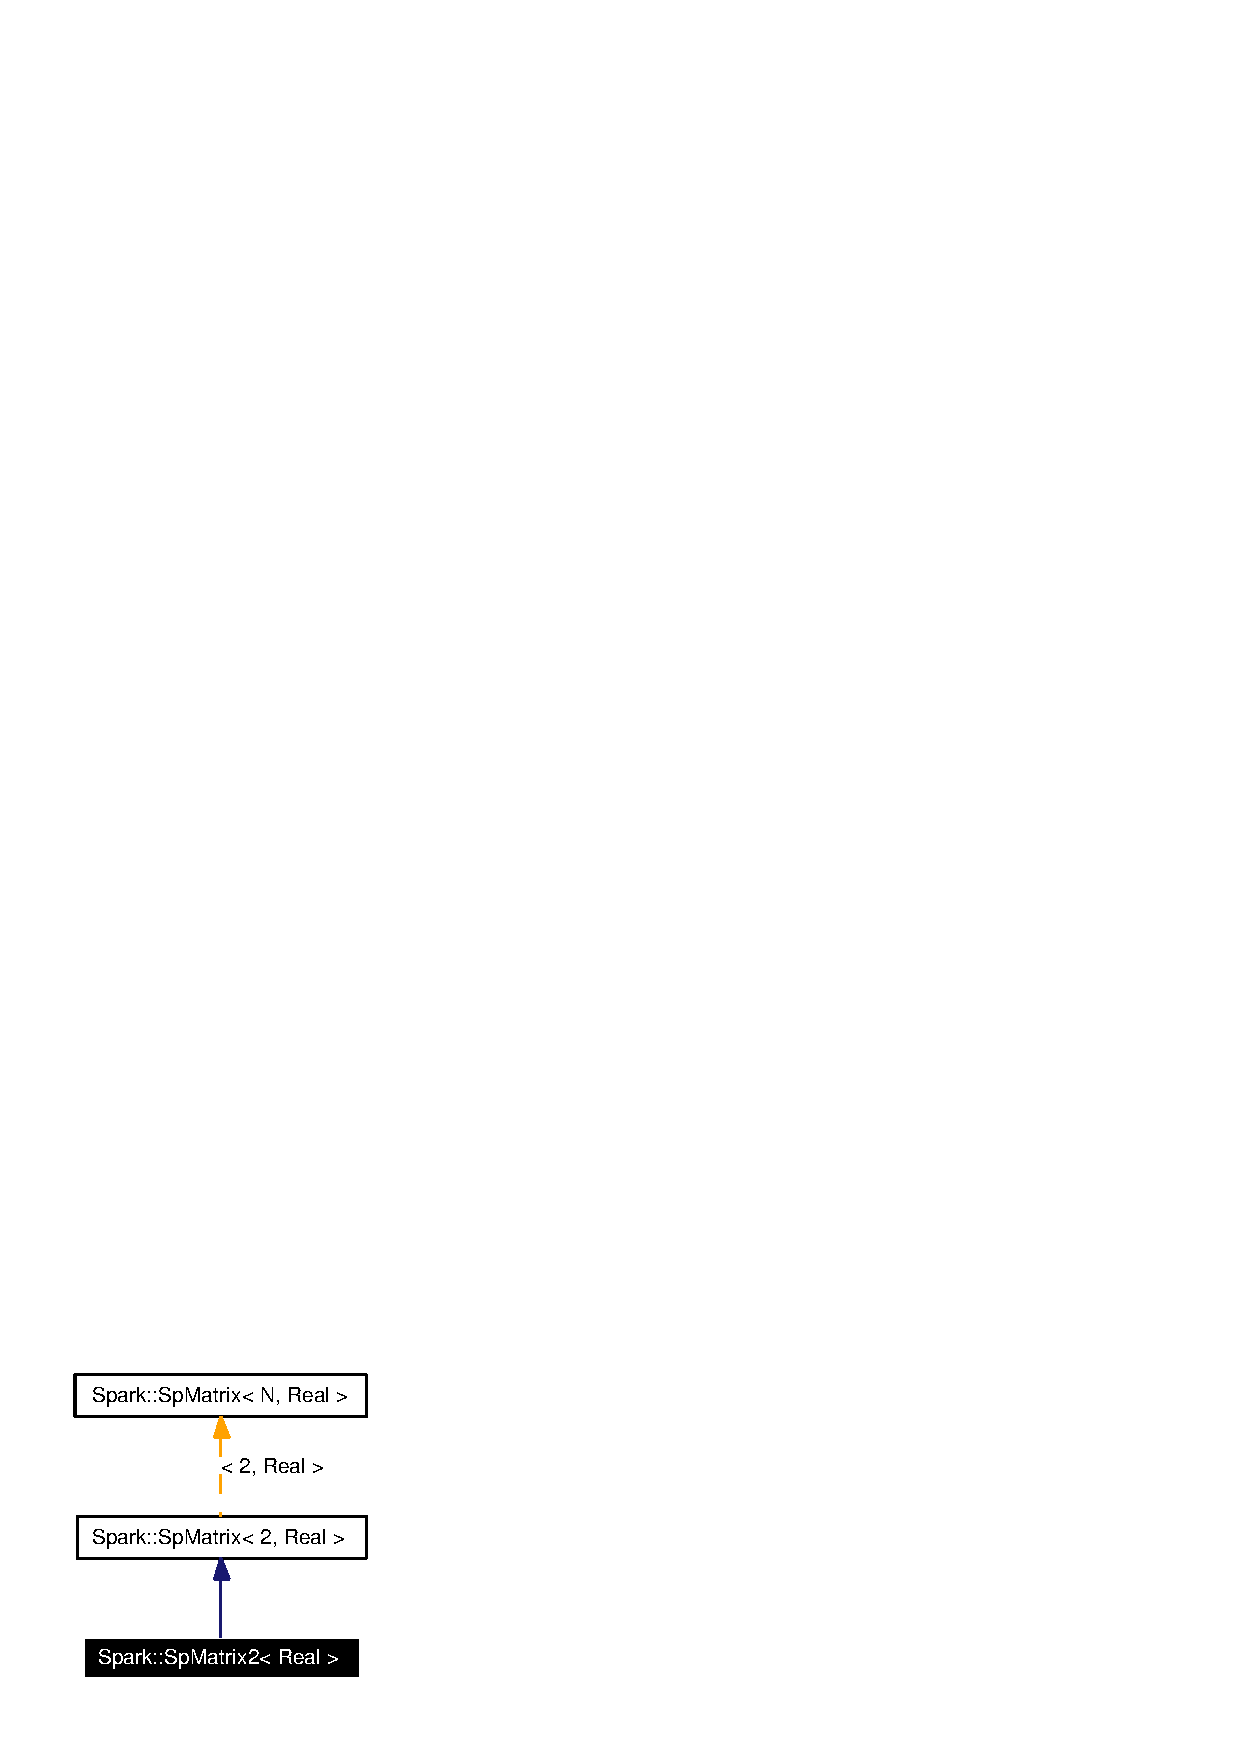
\includegraphics[width=88pt]{classSpark_1_1SpMatrix2__inherit__graph}
\end{center}
\end{figure}
Collaboration diagram for Spark::Sp\-Matrix2$<$ Real $>$:\begin{figure}[H]
\begin{center}
\leavevmode
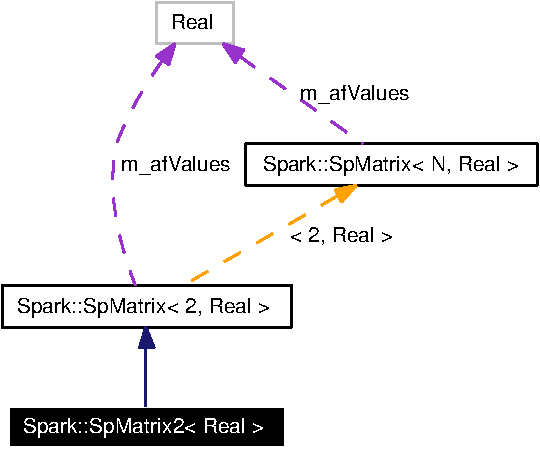
\includegraphics[width=147pt]{classSpark_1_1SpMatrix2__coll__graph}
\end{center}
\end{figure}


\subsection{Detailed Description}
\subsubsection*{template$<$class Real$>$ class Spark::Sp\-Matrix2$<$ Real $>$}

2x2 p\-Matrix class for vector algebra 

Definition at line 106 of file Sp\-Matrix.h.\subsection*{Public Member Functions}
\begin{CompactItemize}
\item 
{\bf Sp\-Matrix2} ()
\item 
{\bf Sp\-Matrix2} (const {\bf Sp\-Matrix2} \&rk\-M)
\item 
{\bf Sp\-Matrix2} (const {\bf Sp\-Matrix}$<$ 2, Real $>$ \&rk\-M)
\item 
{\bf Sp\-Matrix2} (Real f\-M00, Real f\-M01, Real f\-M10, Real f\-M11)
\item 
{\bf Sp\-Matrix2} (const Real af\-Entry[4], bool b\-Row\-Major)
\item 
{\bf Sp\-Matrix2} (const {\bf Sp\-Tuple2}$<$ Real $>$ \&rk\-U, const {\bf Sp\-Tuple2}$<$ Real $>$ \&rk\-V, bool b\-Columns)
\item 
{\bf Sp\-Matrix2} (const {\bf Sp\-Tuple2}$<$ Real $>$ $\ast$ak\-V, bool b\-Columns)
\item 
{\bf Sp\-Matrix2} (Real f\-M00, Real f\-M11)
\item 
{\bf Sp\-Matrix2} (Real f\-Angle)
\item 
{\bf Sp\-Matrix2} \& {\bf operator=} (const {\bf Sp\-Matrix2} \&rk\-M)
\item 
{\bf Sp\-Matrix2} \& {\bf operator=} (const {\bf Sp\-Matrix}$<$ 2, Real $>$ \&rk\-M)
\end{CompactItemize}


\subsection{Constructor \& Destructor Documentation}
\index{Spark::SpMatrix2@{Spark::Sp\-Matrix2}!SpMatrix2@{SpMatrix2}}
\index{SpMatrix2@{SpMatrix2}!Spark::SpMatrix2@{Spark::Sp\-Matrix2}}
\subsubsection{\setlength{\rightskip}{0pt plus 5cm}template$<$class Real$>$ {\bf Spark::Sp\-Matrix2}$<$ Real $>$::{\bf Sp\-Matrix2} ()}\label{classSpark_1_1SpMatrix2_a0}


\index{Spark::SpMatrix2@{Spark::Sp\-Matrix2}!SpMatrix2@{SpMatrix2}}
\index{SpMatrix2@{SpMatrix2}!Spark::SpMatrix2@{Spark::Sp\-Matrix2}}
\subsubsection{\setlength{\rightskip}{0pt plus 5cm}template$<$class Real$>$ {\bf Spark::Sp\-Matrix2}$<$ Real $>$::{\bf Sp\-Matrix2} (const {\bf Sp\-Matrix2}$<$ Real $>$ \& {\em rk\-M})}\label{classSpark_1_1SpMatrix2_a1}


\index{Spark::SpMatrix2@{Spark::Sp\-Matrix2}!SpMatrix2@{SpMatrix2}}
\index{SpMatrix2@{SpMatrix2}!Spark::SpMatrix2@{Spark::Sp\-Matrix2}}
\subsubsection{\setlength{\rightskip}{0pt plus 5cm}template$<$class Real$>$ {\bf Spark::Sp\-Matrix2}$<$ Real $>$::{\bf Sp\-Matrix2} (const {\bf Sp\-Matrix}$<$ 2, Real $>$ \& {\em rk\-M})}\label{classSpark_1_1SpMatrix2_a2}


\index{Spark::SpMatrix2@{Spark::Sp\-Matrix2}!SpMatrix2@{SpMatrix2}}
\index{SpMatrix2@{SpMatrix2}!Spark::SpMatrix2@{Spark::Sp\-Matrix2}}
\subsubsection{\setlength{\rightskip}{0pt plus 5cm}template$<$class Real$>$ {\bf Spark::Sp\-Matrix2}$<$ Real $>$::{\bf Sp\-Matrix2} (Real {\em f\-M00}, Real {\em f\-M01}, Real {\em f\-M10}, Real {\em f\-M11})}\label{classSpark_1_1SpMatrix2_a3}


\index{Spark::SpMatrix2@{Spark::Sp\-Matrix2}!SpMatrix2@{SpMatrix2}}
\index{SpMatrix2@{SpMatrix2}!Spark::SpMatrix2@{Spark::Sp\-Matrix2}}
\subsubsection{\setlength{\rightskip}{0pt plus 5cm}template$<$class Real$>$ {\bf Spark::Sp\-Matrix2}$<$ Real $>$::{\bf Sp\-Matrix2} (const Real {\em af\-Entry}[4], bool {\em b\-Row\-Major})}\label{classSpark_1_1SpMatrix2_a4}


\index{Spark::SpMatrix2@{Spark::Sp\-Matrix2}!SpMatrix2@{SpMatrix2}}
\index{SpMatrix2@{SpMatrix2}!Spark::SpMatrix2@{Spark::Sp\-Matrix2}}
\subsubsection{\setlength{\rightskip}{0pt plus 5cm}template$<$class Real$>$ {\bf Spark::Sp\-Matrix2}$<$ Real $>$::{\bf Sp\-Matrix2} (const {\bf Sp\-Tuple2}$<$ Real $>$ \& {\em rk\-U}, const {\bf Sp\-Tuple2}$<$ Real $>$ \& {\em rk\-V}, bool {\em b\-Columns})}\label{classSpark_1_1SpMatrix2_a5}


\index{Spark::SpMatrix2@{Spark::Sp\-Matrix2}!SpMatrix2@{SpMatrix2}}
\index{SpMatrix2@{SpMatrix2}!Spark::SpMatrix2@{Spark::Sp\-Matrix2}}
\subsubsection{\setlength{\rightskip}{0pt plus 5cm}template$<$class Real$>$ {\bf Spark::Sp\-Matrix2}$<$ Real $>$::{\bf Sp\-Matrix2} (const {\bf Sp\-Tuple2}$<$ Real $>$ $\ast$ {\em ak\-V}, bool {\em b\-Columns})}\label{classSpark_1_1SpMatrix2_a6}


\index{Spark::SpMatrix2@{Spark::Sp\-Matrix2}!SpMatrix2@{SpMatrix2}}
\index{SpMatrix2@{SpMatrix2}!Spark::SpMatrix2@{Spark::Sp\-Matrix2}}
\subsubsection{\setlength{\rightskip}{0pt plus 5cm}template$<$class Real$>$ {\bf Spark::Sp\-Matrix2}$<$ Real $>$::{\bf Sp\-Matrix2} (Real {\em f\-M00}, Real {\em f\-M11})}\label{classSpark_1_1SpMatrix2_a7}


\index{Spark::SpMatrix2@{Spark::Sp\-Matrix2}!SpMatrix2@{SpMatrix2}}
\index{SpMatrix2@{SpMatrix2}!Spark::SpMatrix2@{Spark::Sp\-Matrix2}}
\subsubsection{\setlength{\rightskip}{0pt plus 5cm}template$<$class Real$>$ {\bf Spark::Sp\-Matrix2}$<$ Real $>$::{\bf Sp\-Matrix2} (Real {\em f\-Angle})}\label{classSpark_1_1SpMatrix2_a8}




\subsection{Member Function Documentation}
\index{Spark::SpMatrix2@{Spark::Sp\-Matrix2}!operator=@{operator=}}
\index{operator=@{operator=}!Spark::SpMatrix2@{Spark::Sp\-Matrix2}}
\subsubsection{\setlength{\rightskip}{0pt plus 5cm}template$<$class Real$>$ {\bf Sp\-Matrix2}\& {\bf Spark::Sp\-Matrix2}$<$ Real $>$::operator= (const {\bf Sp\-Matrix}$<$ 2, Real $>$ \& {\em rk\-M})}\label{classSpark_1_1SpMatrix2_a10}


\index{Spark::SpMatrix2@{Spark::Sp\-Matrix2}!operator=@{operator=}}
\index{operator=@{operator=}!Spark::SpMatrix2@{Spark::Sp\-Matrix2}}
\subsubsection{\setlength{\rightskip}{0pt plus 5cm}template$<$class Real$>$ {\bf Sp\-Matrix2}\& {\bf Spark::Sp\-Matrix2}$<$ Real $>$::operator= (const {\bf Sp\-Matrix2}$<$ Real $>$ \& {\em rk\-M})}\label{classSpark_1_1SpMatrix2_a9}




The documentation for this class was generated from the following file:\begin{CompactItemize}
\item 
{\bf Sp\-Matrix.h}\end{CompactItemize}
